% Owner: Hassan Ashraf 24L3073
\section{Problem Definition}
\label{sec:problem}

\subsection{Problem Statement}

Businesses that make products from metals, such as jewellers, electronics
assemblers and metal fabricators, buy their raw materials at prices they do not
control. These prices are set on commodity exchanges such as COMEX and change
every trading day. Our own data (Figure~\ref{fig:raw-prices-p1}) shows how large
these changes are: gold futures traded at about \$1,050 per ounce in late 2015
and rose above \$5,000 per ounce in early 2026, while copper roughly tripled
from its 2016 low. Movements over a single day can also be severe: the largest
one-day falls in our 2010--2026 data are $-10.8\%$ for gold, $-22.3\%$ for
copper and $-31.3\%$ for silver.

For a buyer, this volatility creates two practical problems:

\begin{itemize}
  \item \textbf{Timing.} Most small and medium-sized businesses buy when stock
        runs low or on a fixed schedule, at whatever the price is that day.
        Buying a few weeks earlier or later can change the cost of the same
        order by several percent, which can be the whole profit margin.
  \item \textbf{Judging a supplier's quote.} Suppliers quote the market price
        plus a markup. Without a view of where the price is likely to go, the
        buyer cannot tell whether a quote is fair, generous or inflated.
\end{itemize}

Large firms handle this with in-house analysts and hedging desks. Smaller firms
usually rely on intuition, news headlines or the supplier's own advice, which
is not neutral.

\textbf{ProcurePulse} addresses this gap. It forecasts gold and other metal
prices from COMEX data, gives each forecast a \emph{prediction interval} (a
range the price is expected to fall within, with a stated probability), and
compares a supplier's quote against that forecast to recommend one of three
actions: \textbf{Buy} (the quote is good relative to the expected price),
\textbf{Hold} (prices are expected to fall, so waiting is likely cheaper) or
\textbf{Negotiate} (the quote is high relative to the forecast range).

\begin{figure}[H]
  \centering
  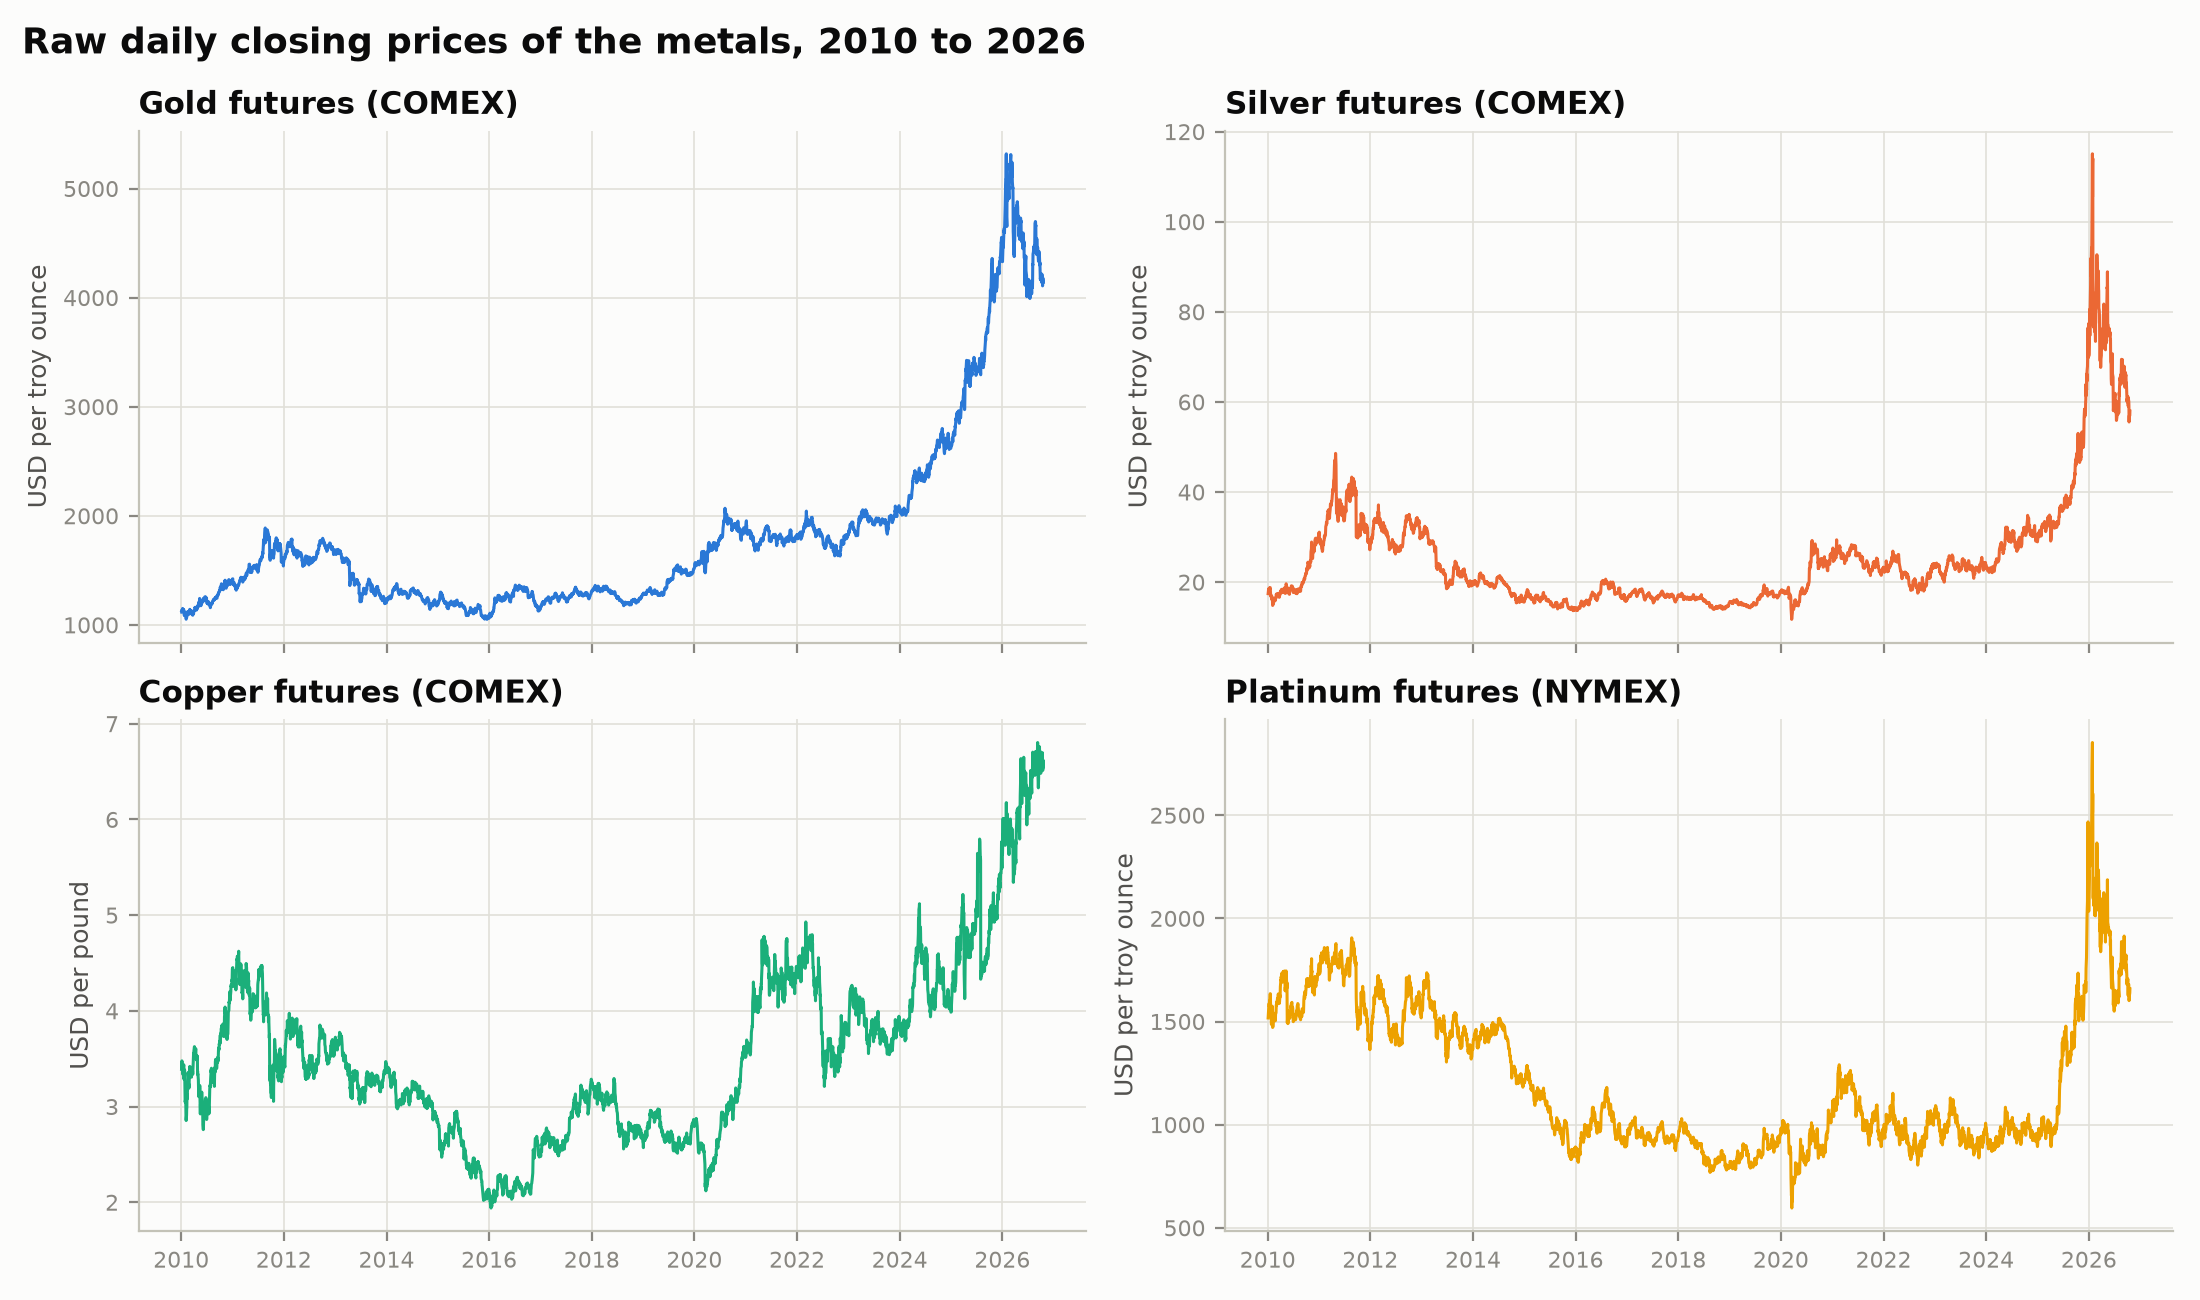
\includegraphics[width=\textwidth]{raw/raw_metal_prices.png}
  \caption{Daily closing prices of COMEX gold, silver and copper futures and
           NYMEX platinum futures, January 2010 to October 2026 (raw data).}
  \label{fig:raw-prices-p1}
\end{figure}

\subsection{Target Audience}

The primary users are \textbf{procurement managers and owners of small and
medium-sized enterprises (SMEs) that buy metals regularly} but do not have
their own market analysts:

\begin{itemize}
  \item jewellery manufacturers and gold traders (gold, silver, platinum);
  \item electronics and electrical-goods assemblers (copper, gold, silver);
  \item metal fabricators and workshops (copper).
\end{itemize}

\textbf{Example user (hypothetical).} Sara manages purchasing for a 40-person jewellery
workshop that buys about 2\,kg of gold each month. Each week she receives
quotes from two suppliers and must decide whether to accept one, wait or push
for a lower price. She has no time to follow the markets in detail. ProcurePulse
gives her a forecast with a clear range and a one-word recommendation she can
act on.

A secondary audience is students and analysts who want a transparent,
reproducible comparison of forecasting models for commodity prices, including
whether external economic signals improve accuracy.

\subsection{AI Justification}

A rule-based system would encode fixed instructions such as ``buy when the
price falls 5\% below its 30-day average''. Such rules fail for this problem
for four reasons:

\begin{enumerate}
  \item \textbf{The patterns are not fixed.} Metal prices move through
        different regimes: long calm periods, sharp trends and sudden shocks
        (for example March 2020 and early 2026 in Figure~\ref{fig:raw-prices-p1}).
        A threshold that works in one regime fails in the next, and someone
        would have to keep rewriting the rules by hand.
  \item \textbf{Many signals interact.} Gold tends to move against the US
        dollar and real interest rates, while oil prices and inflation also
        play a role. The strength of these relationships changes over time
        and is non-linear, which is very hard to express as hand-written rules.
  \item \textbf{Uncertainty must be measured, not guessed.} The
        Buy/Hold/Negotiate decision depends on how likely the price is to move,
        not only on a single predicted value. Statistical and machine learning
        models can learn this uncertainty from historical data and express it
        as a prediction interval; a fixed rule cannot.
  \item \textbf{The data is large and keeps growing.} More than 4,000 trading
        days across eight series are far too many for a person to turn into
        reliable rules, while a model can be retrained automatically as new
        data arrives.
\end{enumerate}

We therefore treat price forecasting as a \textbf{supervised time-series
learning problem}. In later deliverables we will compare models of increasing
complexity on the same chronological train/validation/test split:
\begin{itemize}
  \item a \textbf{naive baseline} (tomorrow's price equals today's) and
        \textbf{ARIMA}, a classical statistical model~\cite{a_box2015};
  \item \textbf{Prophet}~\cite{a_taylor2018} and the gradient-boosted tree
        model \textbf{XGBoost}~\cite{a_chen2016};
  \item a \textbf{Long Short-Term Memory (LSTM)} recurrent neural
        network~\cite{a_hochreiter1997}, which can learn longer-range patterns
        in sequences.
\end{itemize}
Each model will be evaluated with standard forecasting error measures and the
coverage of its prediction intervals~\cite{a_hyndman2021}, with and without the
external signals, to test whether those signals actually improve accuracy. The
approach is only worth using if the learned models beat the naive baseline,
and this comparison is what will show it.